\documentclass[../chapter01.tex]{subfile}

\begin{document}

\begin{Definition}{Brownian Motion}
{\bf Brownian Motion} is a stochastic process $B_t(\omega)$ for $0\le t \le 1$ on a probability space $(\Omega, \Fcal, \Pr)$ such that 
\begin{itemize}
  \item $B_0 = 0$ almost surely.
  \item For $0\le t_0 < t_1 < \ldots < t_n \le 1$ the increments $B_{t_i} - B_{t_{i-1}}$ are independent with law $\Ncal(0, t_{i}-t_{i-1})$.
  \item The function $t \to B_t(\omega)$ is continuous almost surely.
\end{itemize}
\end{Definition}

Let $B_t$ be a Brownian Motion (BM). Then the image measure of $\Pr$ under the map $\Omega\mapsto C[0, 1]$ given by $\omega \mapsto B_{t}(\omega)$ is called the {\bf Wiener measure}.
The Wiener measure is a probability measure on the space $(C[0, 1], \Fcal)$ where $\Fcal = \sigma(\pi_t: 0 \le t \le 1)$, where $\pi_t$ are the projections of a 
function at a given time $t$, i.e. $\pi_t(f) = f(t)$ for all $f \in C[0, 1]$. 

There are two interpretations:
\begin{itemize}
  \item $t \to B_t(\omega)$ for fixed $\omega$: a sample path of random evolution in time
  \item $\omega \to B_t(\omega)$: a random variable taking values in $C[0, 1]$
\end{itemize}

\begin{proposition}
Brownian motion exists
\end{proposition}

There are different proofs of the existence of Brownian motion. This one works by constructing linear interpolations:
\begin{proof}
Let $D_n = \{\frac{k}{2^n} : 0 \le k \le 2^{n}\}$ by dyadic rationals of order $n$. Let $D = \bigcup_n D_n$, and $(\Omega, \Fcal, \Pr)$ a probability space such that $\{Z_{t}: t\in D\}$ are iid 
standard Gaussians. 

Let $B_0 = 0$ and $B_1 = Z_1$\ldots   
\end{proof}

We say that a stochastic process $V_t$ is a {\bf Gaussian process} if for all $t_1 < t_2 <\ldots < t_{n}$ the vector $(V_{t_1},\ldots, V_{t_n})$ is a Gaussian random vector. 
For example, any Brownian motion is a Gaussian process. 

\begin{Figure}
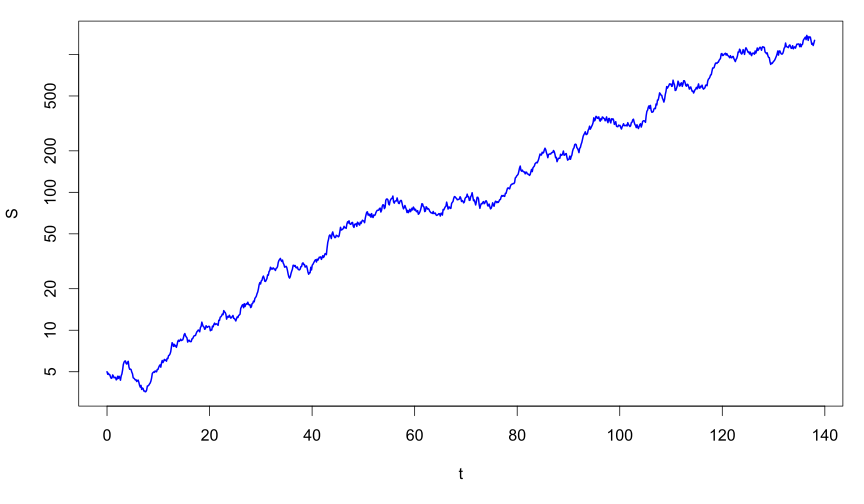
\includegraphics{./figures/BM.svg}
\caption{Example Brownian Motion Path}
\end{Figure}
\end{document}
